  \subsection{Implémentation}
  \begin{frame}
   \frametitle{Procédure de lancement de la détection}
   Le traçage de la fenêtre par l'utilisateur (si nécessaire), puis un clic sur
   \newline le bouton démarrer entraîne :
   \begin{figure}[H]
 \centering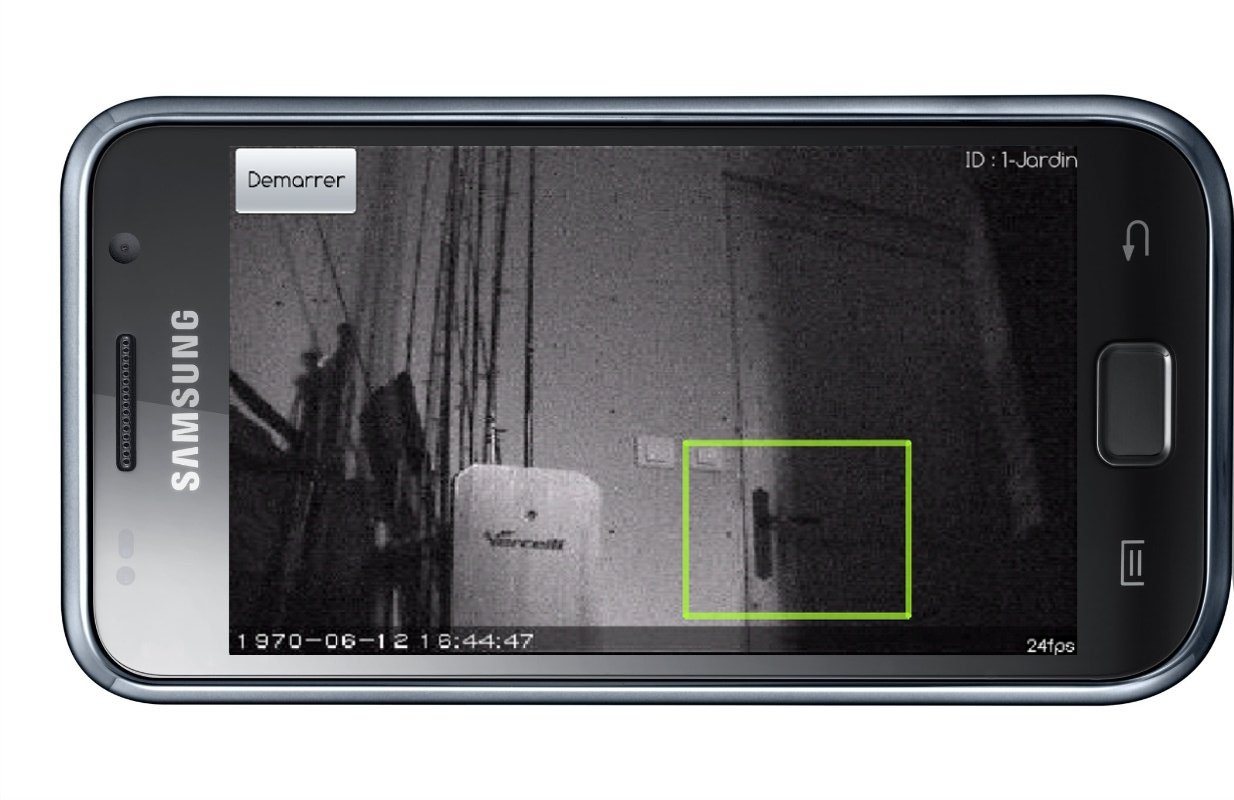
\includegraphics[scale=0.10]{Images/samsung-galaxy-s-vue3.jpg}
      \end{figure}
    \begin{enumerate}
    \item Demande d'ajout d'une fenêtre de détection auprès de la caméra
    \item Détéction de la présence d'une eventuelle fenêtre personnalisée puis
    mise à jours de ses coordonnées en cas de présence
    \item Démarrage de la tache du service :
     \begin{enumerate}
       \item Ajout notification ``En-Cours''
       \item Démarrage d'un thread chargé d'analyser le niveau de détection
       retourné par la caméra
       \end{enumerate}
   \end{enumerate}
  \end{frame}